\documentclass[11pt,a4paper]{article}
\usepackage{mystyle}
\usepackage{schueler}
%\usepackage{lehrer}


\usepackage{circuitikz}

\author{}
\title{Optische Abbildungen}

\begin{document}
\maketitle

%\thispagestyle{empty}

\section{Einleitung}
In diesem Praktikumsversuch sollen optische Abbildungen untersucht werden.
Dazu werden wir Gegenstände mit Hilfe einer Sammellinse auf einem Schirm abbilden.
Wir werden die Vergrösserung des Bildes untersuchen und die Linsengleichung
bestätigen.

\section{Versuchsaufbau}

\begin{figure}[h]
	\begin{center}
	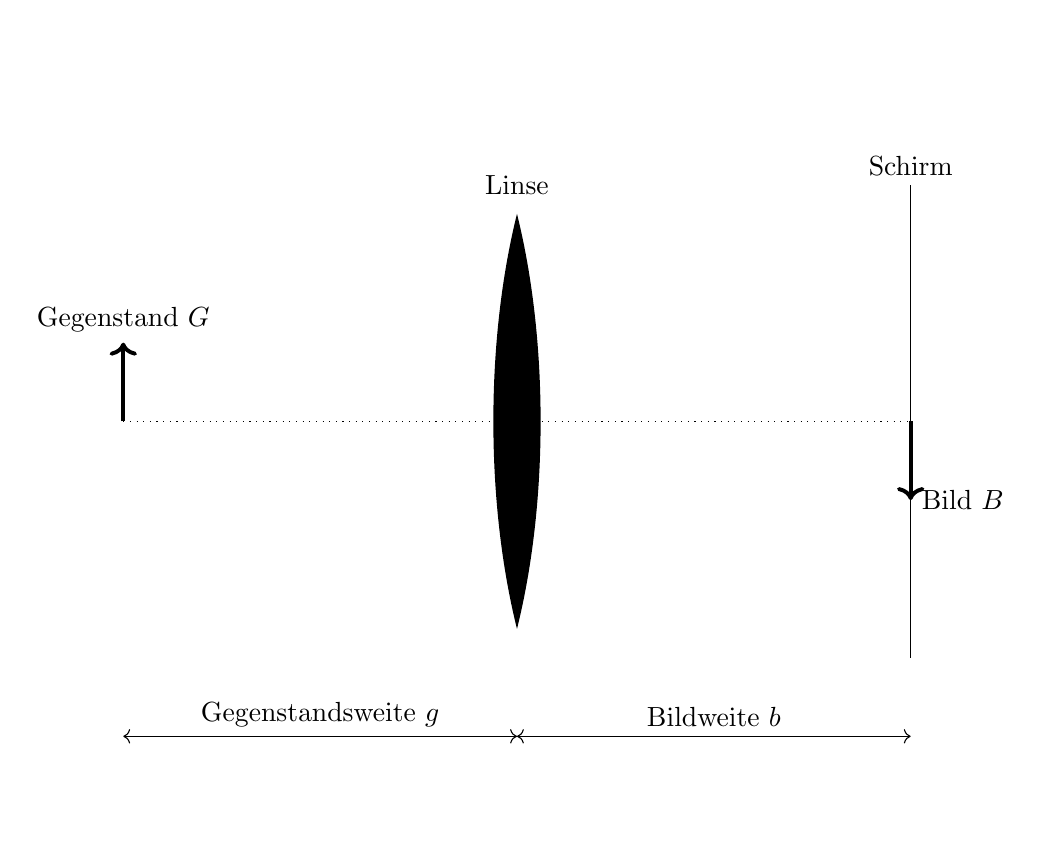
\begin{tikzpicture}

%Mittellinie
\draw [dotted] (-5,0)--(5,0);

%Gegenstand
\draw [->=latex, line width=0.05cm] (-5,0)--(-5,1) node [above] {Gegenstand $G$};
%Bild
\draw [->=latex, line width=0.05cm] (5,0)--(5,-1) node [right] {Bild $B$};

\begin{scope}[xscale=2, yscale=5]
\clip (-0.85,0) circle (1cm);
\clip (0.85,0) circle (1cm);
\fill(-2,-2) rectangle (2,2);
\end{scope}

\draw (0,3) node {Linse};

%Schirm
\draw (5,-3)--(5,3) node [above] {Schirm};


\draw [<->=latex] (-5,-4)--(0,-4) node [midway, above] {Gegenstandsweite $g$};
\draw [<->=latex] (0,-4)--(5,-4) node [midway, above] {Bildweite $b$};
\end{tikzpicture}
	\caption{\label{fig1} Skizze des Versuchsaufbaus.} 
	\end{center}
\end{figure}

Auf eine optische Bank wird eine Halogenlampe, eine Linse und ein Schirm montiert.
Dabei dient die Halogenlampe im ersten Teil als Gegenstand $G$.
Das Bild $B$ wird auf den Schirm abgebildet.
Der Abstand zwischen Gegenstand und Linse heisst Gegenstandsweite $g$, der Abstand zwischen
Linse und Schirm heisst Bildweite $b$.
Die Linse hat eine Brennweite $f$.

\section{Versuch}

Für den ersten Versuch variieren wir die Gegenstandsweite und messen die Bildweite.
Ausserdem messen wir die Grösse des Bildes $B$. Alle Messwerte sind links in Tabelle \ref{tab1} angegeben.
Im rechten Teil der Tabelle \ref{tab1} wurden die Messdaten schon ausgewertet. 

\begin{table}
\begin{center}
\begin{tabular}{ccc|cccc}
	\multicolumn{3}{c}{Messung} & \multicolumn{4}{c}{Auswertung}\\
$g$ (cm) & $b$ (cm) &   $B$ (cm)   & $1/g$ (1/cm) & $1/b$ (1/cm) &  $b/g$   & $B/G$\\\hline
13   &   43     &   1.3      & 0.076923   & 0.02325    & 3.30769  &3.25 \\
15   &   30     &   0.8      & 0.066667   & 0.03333    & 2        &2    \\
20   &   19.3   &   0.5      & 0.050000   & 0.05181    & 0.965    &1.25 \\
21   &   18.5   &   0.5      & 0.047619   & 0.05405    & 0.880952 &1.25 \\
23   &   17     &   0.4      & 0.043478   & 0.05882    & 0.73913  &1 \\
30   &   14.5   &   0.4      & 0.033333   & 0.06896    & 0.483333 &1\\
\end{tabular}
\caption{\label{tab1}
Für diese Messreihe wurde die Linse mit der Brennweite $f=\SI{10}{cm}$ verwandt. 
Im linken Teil der Tabelle stehen Messwerte, rechts wurden die Daten schon bearbeitet.
}
\end{center}
\end{table}

\subsection{Vergrösserung}
\begin{figure}[h]
\begin{tikzpicture}[gnuplot]
%% generated with GNUPLOT 4.6p1 (Lua 5.1; terminal rev. 99, script rev. 100)
%% Don 14 Mär 2013 14:38:57 CET
\tikzset{every node/.append style={font={\sffamily\fontsize{12pt}{14.4pt}\selectfont}}}
\path (0.000,0.000) rectangle (14.100,10.000);
\gpcolor{color=gp lt color border}
\gpsetlinetype{gp lt border}
\gpsetlinewidth{1.00}
\draw[gp path] (1.806,1.184)--(1.986,1.184);
\draw[gp path] (13.436,1.184)--(13.256,1.184);
\node[gp node right] at (1.585,1.184) { 0};
\draw[gp path] (1.806,2.380)--(1.986,2.380);
\draw[gp path] (13.436,2.380)--(13.256,2.380);
\node[gp node right] at (1.585,2.380) { 0.5};
\draw[gp path] (1.806,3.576)--(1.986,3.576);
\draw[gp path] (13.436,3.576)--(13.256,3.576);
\node[gp node right] at (1.585,3.576) { 1};
\draw[gp path] (1.806,4.772)--(1.986,4.772);
\draw[gp path] (13.436,4.772)--(13.256,4.772);
\node[gp node right] at (1.585,4.772) { 1.5};
\draw[gp path] (1.806,5.969)--(1.986,5.969);
\draw[gp path] (13.436,5.969)--(13.256,5.969);
\node[gp node right] at (1.585,5.969) { 2};
\draw[gp path] (1.806,7.165)--(1.986,7.165);
\draw[gp path] (13.436,7.165)--(13.256,7.165);
\node[gp node right] at (1.585,7.165) { 2.5};
\draw[gp path] (1.806,8.361)--(1.986,8.361);
\draw[gp path] (13.436,8.361)--(13.256,8.361);
\node[gp node right] at (1.585,8.361) { 3};
\draw[gp path] (1.806,9.557)--(1.986,9.557);
\draw[gp path] (13.436,9.557)--(13.256,9.557);
\node[gp node right] at (1.585,9.557) { 3.5};
\draw[gp path] (1.806,1.184)--(1.806,1.364);
\draw[gp path] (1.806,9.557)--(1.806,9.377);
\node[gp node center] at (1.806,0.814) { 0};
\draw[gp path] (3.467,1.184)--(3.467,1.364);
\draw[gp path] (3.467,9.557)--(3.467,9.377);
\node[gp node center] at (3.467,0.814) { 0.5};
\draw[gp path] (5.129,1.184)--(5.129,1.364);
\draw[gp path] (5.129,9.557)--(5.129,9.377);
\node[gp node center] at (5.129,0.814) { 1};
\draw[gp path] (6.790,1.184)--(6.790,1.364);
\draw[gp path] (6.790,9.557)--(6.790,9.377);
\node[gp node center] at (6.790,0.814) { 1.5};
\draw[gp path] (8.452,1.184)--(8.452,1.364);
\draw[gp path] (8.452,9.557)--(8.452,9.377);
\node[gp node center] at (8.452,0.814) { 2};
\draw[gp path] (10.113,1.184)--(10.113,1.364);
\draw[gp path] (10.113,9.557)--(10.113,9.377);
\node[gp node center] at (10.113,0.814) { 2.5};
\draw[gp path] (11.775,1.184)--(11.775,1.364);
\draw[gp path] (11.775,9.557)--(11.775,9.377);
\node[gp node center] at (11.775,0.814) { 3};
\draw[gp path] (13.436,1.184)--(13.436,1.364);
\draw[gp path] (13.436,9.557)--(13.436,9.377);
\node[gp node center] at (13.436,0.814) { 3.5};
\draw[gp path] (1.806,9.557)--(1.806,1.184)--(13.436,1.184)--(13.436,9.557)--cycle;
\node[gp node center,rotate=-270] at (0.295,5.370) {$\frac{B}{G}$};
\node[gp node center] at (7.621,0.259) {$\frac{b}{g}$};
\node[gp node right] at (3.574,9.192) {Daten};
\gpcolor{rgb color={0.000,0.000,0.000}}
\gpsetlinewidth{2.00}
\gpsetpointsize{4.00}
\gppoint{gp mark 6}{(12.797,8.959)}
\gppoint{gp mark 6}{(8.452,5.969)}
\gppoint{gp mark 6}{(5.013,4.174)}
\gppoint{gp mark 6}{(4.733,4.174)}
\gppoint{gp mark 6}{(4.262,3.576)}
\gppoint{gp mark 6}{(3.412,3.576)}
\gppoint{gp mark 6}{(4.327,9.192)}
\gpcolor{color=gp lt color border}
\node[gp node right] at (3.574,8.822) {Theorie};
\gpcolor{rgb color={0.000,0.000,0.000}}
\gpsetlinetype{gp lt plot 0}
\draw[gp path] (3.795,8.822)--(4.859,8.822);
\draw[gp path] (3.412,2.340)--(3.507,2.409)--(3.602,2.477)--(3.696,2.545)--(3.791,2.613)%
  --(3.886,2.682)--(3.981,2.750)--(4.076,2.818)--(4.170,2.886)--(4.265,2.955)--(4.360,3.023)%
  --(4.455,3.091)--(4.550,3.159)--(4.644,3.228)--(4.739,3.296)--(4.834,3.364)--(4.929,3.432)%
  --(5.024,3.501)--(5.118,3.569)--(5.213,3.637)--(5.308,3.705)--(5.403,3.774)--(5.498,3.842)%
  --(5.592,3.910)--(5.687,3.978)--(5.782,4.047)--(5.877,4.115)--(5.972,4.183)--(6.066,4.251)%
  --(6.161,4.319)--(6.256,4.388)--(6.351,4.456)--(6.446,4.524)--(6.540,4.592)--(6.635,4.661)%
  --(6.730,4.729)--(6.825,4.797)--(6.920,4.865)--(7.014,4.934)--(7.109,5.002)--(7.204,5.070)%
  --(7.299,5.138)--(7.394,5.207)--(7.488,5.275)--(7.583,5.343)--(7.678,5.411)--(7.773,5.480)%
  --(7.868,5.548)--(7.962,5.616)--(8.057,5.684)--(8.152,5.753)--(8.247,5.821)--(8.342,5.889)%
  --(8.436,5.957)--(8.531,6.026)--(8.626,6.094)--(8.721,6.162)--(8.815,6.230)--(8.910,6.299)%
  --(9.005,6.367)--(9.100,6.435)--(9.195,6.503)--(9.289,6.572)--(9.384,6.640)--(9.479,6.708)%
  --(9.574,6.776)--(9.669,6.845)--(9.763,6.913)--(9.858,6.981)--(9.953,7.049)--(10.048,7.118)%
  --(10.143,7.186)--(10.237,7.254)--(10.332,7.322)--(10.427,7.391)--(10.522,7.459)--(10.617,7.527)%
  --(10.711,7.595)--(10.806,7.664)--(10.901,7.732)--(10.996,7.800)--(11.091,7.868)--(11.185,7.937)%
  --(11.280,8.005)--(11.375,8.073)--(11.470,8.141)--(11.565,8.210)--(11.659,8.278)--(11.754,8.346)%
  --(11.849,8.414)--(11.944,8.483)--(12.039,8.551)--(12.133,8.619)--(12.228,8.687)--(12.323,8.756)%
  --(12.418,8.824)--(12.513,8.892)--(12.607,8.960)--(12.702,9.029)--(12.797,9.097);
\gpcolor{color=gp lt color border}
\gpsetlinetype{gp lt border}
\gpsetlinewidth{1.00}
\draw[gp path] (1.806,9.557)--(1.806,1.184)--(13.436,1.184)--(13.436,9.557)--cycle;
%% coordinates of the plot area
\gpdefrectangularnode{gp plot 1}{\pgfpoint{1.806cm}{1.184cm}}{\pgfpoint{13.436cm}{9.557cm}}
\end{tikzpicture}
%% gnuplot variables

\caption{\label{fig3} Experimentelle Überprüfung der Vergrösserung durch Gleichung \ref{V} und deren theoretischer Verlauf.} 
\end{figure}

Die Vergrösserung $V$ ist definiert als das Verhältnis der Grösse des Bildes $B$ zur Grösse des Gegenstands $G$.
Das gleiche Verhältnis gilt auch für die Bildweite $b$ und die Gegenstandsweite $g$.
\begin{eqnarray}
	V=\frac{B}{G}=\frac{b}{g}
	\label{V}
\end{eqnarray}

Die Verhältnisse $B/G$ und $b/g$ haben wir in Tabelle \ref{tab1} berechnet. Zur besseren Übersicht haben wir sie auch in
einem Graphen dargestellt (siehe Graph \ref{fig3}). Man sieht, dass Formel \ref{V} für grosse $V$ sehr gut stimmt.
Für kleine $V$ weichen die Messwerte etwas ab. Dies kann damit begründet werden, dass das Bild sehr klein wurde, und damit
Messfehler eine grössere Rolle spielen.


\subsection{Linsengleichung}
Als nächstes wollen wir die Linsengleichung experimentell überprüfen. Für Abbildungen mit Linsen gilt
die Linsengleichung:
\begin{eqnarray}
	\frac{1}{f} = \frac{1}{b} + \frac{1}{g}\text{.}
	\label{L}
\end{eqnarray}
$f$ steht für die Brennweite der Linse.


\begin{figure}[h]
\begin{tikzpicture}[gnuplot]
%% generated with GNUPLOT 4.6p1 (Lua 5.1; terminal rev. 99, script rev. 100)
%% Don 14 Mär 2013 14:38:57 CET
\tikzset{every node/.append style={font={\sffamily\fontsize{12pt}{14.4pt}\selectfont}}}
\path (0.000,0.000) rectangle (14.100,10.000);
\gpcolor{color=gp lt color border}
\gpsetlinetype{gp lt border}
\gpsetlinewidth{1.00}
\draw[gp path] (2.027,1.184)--(2.207,1.184);
\draw[gp path] (13.436,1.184)--(13.256,1.184);
\node[gp node right] at (1.806,1.184) { 0};
\draw[gp path] (2.027,2.859)--(2.207,2.859);
\draw[gp path] (13.436,2.859)--(13.256,2.859);
\node[gp node right] at (1.806,2.859) { 0.02};
\draw[gp path] (2.027,4.533)--(2.207,4.533);
\draw[gp path] (13.436,4.533)--(13.256,4.533);
\node[gp node right] at (1.806,4.533) { 0.04};
\draw[gp path] (2.027,6.208)--(2.207,6.208);
\draw[gp path] (13.436,6.208)--(13.256,6.208);
\node[gp node right] at (1.806,6.208) { 0.06};
\draw[gp path] (2.027,7.882)--(2.207,7.882);
\draw[gp path] (13.436,7.882)--(13.256,7.882);
\node[gp node right] at (1.806,7.882) { 0.08};
\draw[gp path] (2.027,9.557)--(2.207,9.557);
\draw[gp path] (13.436,9.557)--(13.256,9.557);
\node[gp node right] at (1.806,9.557) { 0.1};
\draw[gp path] (2.027,1.184)--(2.027,1.364);
\draw[gp path] (2.027,9.557)--(2.027,9.377);
\node[gp node center] at (2.027,0.814) { 0};
\draw[gp path] (4.309,1.184)--(4.309,1.364);
\draw[gp path] (4.309,9.557)--(4.309,9.377);
\node[gp node center] at (4.309,0.814) { 0.02};
\draw[gp path] (6.591,1.184)--(6.591,1.364);
\draw[gp path] (6.591,9.557)--(6.591,9.377);
\node[gp node center] at (6.591,0.814) { 0.04};
\draw[gp path] (8.872,1.184)--(8.872,1.364);
\draw[gp path] (8.872,9.557)--(8.872,9.377);
\node[gp node center] at (8.872,0.814) { 0.06};
\draw[gp path] (11.154,1.184)--(11.154,1.364);
\draw[gp path] (11.154,9.557)--(11.154,9.377);
\node[gp node center] at (11.154,0.814) { 0.08};
\draw[gp path] (13.436,1.184)--(13.436,1.364);
\draw[gp path] (13.436,9.557)--(13.436,9.377);
\node[gp node center] at (13.436,0.814) { 0.1};
\draw[gp path] (2.027,9.557)--(2.027,1.184)--(13.436,1.184)--(13.436,9.557)--cycle;
\node[gp node center,rotate=-270] at (0.295,5.370) {Reziproke Bildweite $\frac{1}{b}$ (1/cm)};
\node[gp node center] at (7.731,0.259) {Reziproke Gegenstandsweite $\frac{1}{g}$ (1/cm)};
\node[gp node right] at (11.709,9.192) {Daten};
\gpcolor{rgb color={0.000,0.000,0.000}}
\gpsetlinewidth{2.00}
\gpsetpointsize{4.00}
\gppoint{gp mark 6}{(10.803,3.131)}
\gppoint{gp mark 6}{(9.633,3.975)}
\gppoint{gp mark 6}{(7.732,5.522)}
\gppoint{gp mark 6}{(7.460,5.710)}
\gppoint{gp mark 6}{(6.987,6.109)}
\gppoint{gp mark 6}{(5.830,6.958)}
\gppoint{gp mark 6}{(12.462,9.192)}
\gpcolor{color=gp lt color border}
\node[gp node right] at (11.709,8.822) {Linsengleichung};
\gpcolor{rgb color={0.000,0.000,0.000}}
\gpsetlinetype{gp lt plot 0}
\draw[gp path] (11.930,8.822)--(12.994,8.822);
\draw[gp path] (2.027,9.557)--(2.142,9.472)--(2.257,9.388)--(2.373,9.303)--(2.488,9.219)%
  --(2.603,9.134)--(2.718,9.050)--(2.834,8.965)--(2.949,8.880)--(3.064,8.796)--(3.179,8.711)%
  --(3.295,8.627)--(3.410,8.542)--(3.525,8.458)--(3.640,8.373)--(3.756,8.288)--(3.871,8.204)%
  --(3.986,8.119)--(4.101,8.035)--(4.217,7.950)--(4.332,7.865)--(4.447,7.781)--(4.562,7.696)%
  --(4.678,7.612)--(4.793,7.527)--(4.908,7.443)--(5.023,7.358)--(5.139,7.273)--(5.254,7.189)%
  --(5.369,7.104)--(5.484,7.020)--(5.600,6.935)--(5.715,6.851)--(5.830,6.766)--(5.945,6.681)%
  --(6.060,6.597)--(6.176,6.512)--(6.291,6.428)--(6.406,6.343)--(6.521,6.259)--(6.637,6.174)%
  --(6.752,6.089)--(6.867,6.005)--(6.982,5.920)--(7.098,5.836)--(7.213,5.751)--(7.328,5.667)%
  --(7.443,5.582)--(7.559,5.497)--(7.674,5.413)--(7.789,5.328)--(7.904,5.244)--(8.020,5.159)%
  --(8.135,5.074)--(8.250,4.990)--(8.365,4.905)--(8.481,4.821)--(8.596,4.736)--(8.711,4.652)%
  --(8.826,4.567)--(8.942,4.482)--(9.057,4.398)--(9.172,4.313)--(9.287,4.229)--(9.403,4.144)%
  --(9.518,4.060)--(9.633,3.975)--(9.748,3.890)--(9.863,3.806)--(9.979,3.721)--(10.094,3.637)%
  --(10.209,3.552)--(10.324,3.468)--(10.440,3.383)--(10.555,3.298)--(10.670,3.214)--(10.785,3.129)%
  --(10.901,3.045)--(11.016,2.960)--(11.131,2.876)--(11.246,2.791)--(11.362,2.706)--(11.477,2.622)%
  --(11.592,2.537)--(11.707,2.453)--(11.823,2.368)--(11.938,2.283)--(12.053,2.199)--(12.168,2.114)%
  --(12.284,2.030)--(12.399,1.945)--(12.514,1.861)--(12.629,1.776)--(12.745,1.691)--(12.860,1.607)%
  --(12.975,1.522)--(13.090,1.438)--(13.206,1.353)--(13.321,1.269)--(13.436,1.184);
\gpcolor{color=gp lt color border}
\gpsetlinetype{gp lt border}
\gpsetlinewidth{1.00}
\draw[gp path] (2.027,9.557)--(2.027,1.184)--(13.436,1.184)--(13.436,9.557)--cycle;
%% coordinates of the plot area
\gpdefrectangularnode{gp plot 1}{\pgfpoint{2.027cm}{1.184cm}}{\pgfpoint{13.436cm}{9.557cm}}
\end{tikzpicture}
%% gnuplot variables

\caption{\label{fig1} Experimentelle Überprüfung der Linsengleichung (Formel \ref{L}). Zum Vergleich die theoretische Kurve.} 
\end{figure}

In Graph \ref{fig1} ist die reziproke Bildweite $1/b$ über der reziproken Gegenstandsweite $1/g$ dargestellt.
Wir sehen einen linearen Verlauf von $1/b$. Zum Vergleich ist auch die theoretische Kurve, die durch die Linsengleichung (Gleichung \ref{L})
beschrieben wird dargestellt. Man sieht, dass die Messpunkte ausgezeichnet mit der theoretischen Kurve übereinstimmt.

\section{Zusammenfassung}
In diesem Experiment haben wir optische Abbildungen durch Linsen untersucht.
Wir haben überprüft, wie die Vergrösserung $V$ mit Bildweite $b$ und Gegenstandsweite $g$ verknüpft ist. 
Wir konnten den bekannten Zusammenhang $V=b/g$ experimentell bestätigen.
In einer zweiten Auswertung konnten wir die Linsengleichung experimentell bestätigen.


\end{document}
